New market information is constantly becoming available. This fact will have a huge impact on the forecasts but it does not make them less useful if just uncertainty is taken into consideration and represented to the user. The uncertain information "qualifies" the forecast because it makes the user capable of assessing how much the new information will influence the price \cite{EnergyPriceForecasting}.
  
It is necessary to get a complete understanding of uncertainties in the data you wish to present and an adequate way of visualizing it to the user. This becomes even more important when the information is to be used in dynamic environments where high-risk decisions have to be made \cite{UncertainInformation}. Furthermore, new technologies have made it possible to analyze and compare data from multiple sources which can create an information overload that makes decision-making even more difficult. The Decision Support System (DSS) as described above can combine and present all of this information in order to support users in their attempt to make the best decision. However, autonomous systems does not always guarantee the best result or performance. It can actually contribute to creation or exposing of uncertainties when dealing with complex environments such as financial markets \cite{UncertainInformation} if not handled carefully. It necessary to present the uncertain information in the most appropriate way.
\\[0.5cm]
Most people are met with uncertainties on a daily basis. We are fully aware that decisions have to be made even though information is not exact or complete. Often this results in decisions based on guesses and assumptions \cite{UncertainInformation}. When dealing with high-risk decisions it is necessary to be aware of the uncertainties so that it can be accounted for when taking the actual decision. 
There are different types of uncertainties and it can be characterized as both subjective and objective (see figure~\ref{fig:typesOfUncertainty}). 
\begin{figure}[h!]
\centering
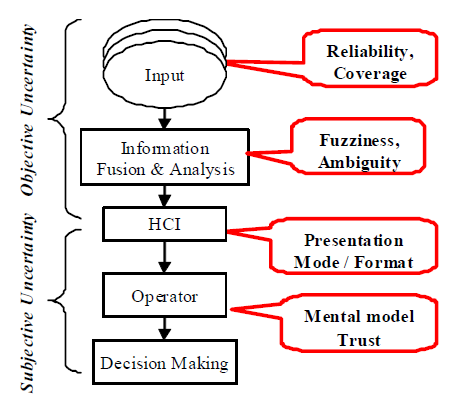
\includegraphics[width=0.7\linewidth,natwidth=898,natheight=587]{billeder/TypesOfUncertainInformation.png}
\caption{Types of uncertainty from \cite{UncertainInformation}}
\label{fig:typesOfUncertainty}
\end{figure}  
The objective uncertainties is the acquisition and processing of the data, and the output. Is the data acquired from a trusted source, is it comprehensive enough and does processing impact the data precision. We are combining and comparing information from different sources during the data processing which can bring uncertainties such as conflicting data or just bad estimates. This information needs to be brought to the users attention so they can act on it. The subjective uncertainties arise in the mind of the user when he is to make a decision. People perceive, interpret and process information differently depending on their background. It is not enough to simply present the information. It is essential to visualize and present the information specifically to the users of the system. Decisions also depend on the specific task, the context, needed accuracy, time constraint, level of risk and experience. 
\\[0.5cm]
Five strategies for user decision making in an uncertain environment is presented in \cite{UncertainInformation}. 
\begin{itemize}
\item Reduction: collecting further information to reduce uncertainty.
\item Assumption-based reasoning: Fill in gaps by relying on experience and imagination, or make sense of factual information.
\item Weighting pros and cons of alternatives
\item Forestalling: Prepare what to do in case of a potential negative result
\item Suppressing uncertainty by simply ignoring it. Last resort.
\end{itemize}  
This emphasizes the need for making the users aware of potential uncertainties in the information e.g. situation awareness. What strategy to use relies greatly on how much uncertainty. The uncertainties should always be made aware to the users so that it is not necessary for them to check the validity themselves. It is furthermore important that the user understands the basic logic of the algorithm so that the answer is not just "black magic". They need to trust it.
\\[0.5cm]
The way of presenting information greatly impacts the decision making process. People can process more data and do it more quickly when it is presented graphically rather than in text \cite{UncertainInformation}. This does not imply that the information can be overloaded with graphical information; it is still important to only show what is most critical for the user to make the best decision. An example of a graphical representation that is perceived quickly is \textit{blurred or degraded graphical images} where the images in a natural way visualizes the amount of uncertainty by blurring it accordingly (see figure ~\ref{fig:blurryIcons}). 
\begin{figure}[h!]
\centering
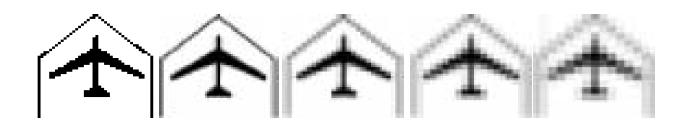
\includegraphics[width=0.7\linewidth,natwidth=898,natheight=587]{billeder/blurryIcons.png}
\caption{Blurry icons from \cite{UncertainInformation}}
\label{fig:blurryIcons}
\end{figure}  
\\[0.5cm]
Based on the discussions in \cite{UncertainInformation} they present a number of high level guidelines for presenting uncertainty. To summarise the most prominent:
\begin{itemize}
\item Always define and present uncertainty and accuracy of data.
\item Present uncertainty at all time and not only when the decision has to be made.
\item Identify the user so that the system can be aligned with their way of reasoning and thinking. This include basic understanding of the underlying algorithm.
\item Provide conflict in data if it is present.
\item Graphical distortion can be improve performance when showing uncertainties.
\item Graphical presentation is not as precise a numerical but they can support each other in achieving precision and performance.
\item Users must be able to restructure the information environment themselves so that it fits their need and way of thinking.
\end{itemize}
The guidelines can be used when developing interface prototypes for Decision Support Systems (DSS).